% ============================================================
% Chapitre 3 : Classification
% ============================================================
\chapter{Classification --- R\'egression Logistique, $k$-NN, Na\"ive Bayes}
\label{ch:classification}

\begin{intuition}[title=\textbf{Du continu au discret}]
Contrairement \`a la r\'egression o\`u $y \in \R$, la classification pr\'edit une
\textbf{\'etiquette discr\`ete} $y \in \{0, 1, \ldots, K-1\}$. Ce chapitre pr\'esente
trois approches fondamentales : la r\'egression logistique (mod\`ele discriminant
param\'etrique), les $k$ plus proches voisins (m\'ethode non-param\'etrique) et
Na\"ive Bayes (mod\`ele g\'en\'eratif).
\end{intuition}

% ============================================================
\section{R\'egression logistique}
\label{sec:logistic}

\subsection{Cas binaire : la fonction sigmo\"ide}

\begin{definition}[Fonction sigmo\"ide]
La fonction sigmo\"ide (ou logistique) est d\'efinie par :
\[
  \sigma(z) = \frac{1}{1 + e^{-z}}, \qquad z \in \R
\]
Elle v\'erifie : $\sigma(-z) = 1 - \sigma(z)$ et $\sigma'(z) = \sigma(z)(1 - \sigma(z))$.
\end{definition}

Le mod\`ele de r\'egression logistique binaire pose :
\[
  P(Y = 1 \mid \bm{x}) = \sigma(\bm{w}^\top \bm{x} + b)
  = \frac{1}{1 + \exp(-\bm{w}^\top \bm{x} - b)}
\]
o\`u $\bm{w} \in \R^p$ est le vecteur de poids et $b \in \R$ le biais.

\begin{formules}[title=\textbf{Log-odds (logit)}]
\[
  \log \frac{P(Y=1 \mid \bm{x})}{P(Y=0 \mid \bm{x})}
  = \bm{w}^\top \bm{x} + b
\]
La fronti\`ere de d\'ecision est l'hyperplan $\{\bm{x} : \bm{w}^\top \bm{x} + b = 0\}$.
\end{formules}

\subsection{Estimation par maximum de vraisemblance}

\begin{theoreme}[Vraisemblance de la r\'egression logistique]
\label{thm:logistic-mle}
\'Etant donn\'e $n$ observations $(\bm{x}_i, y_i)$ avec $y_i \in \{0, 1\}$,
la log-vraisemblance est :
\[
  \ell(\bm{w}, b) = \sum_{i=1}^{n} \Bigl[
    y_i \log \sigma(\bm{w}^\top \bm{x}_i + b)
    + (1 - y_i) \log\bigl(1 - \sigma(\bm{w}^\top \bm{x}_i + b)\bigr)
  \Bigr]
\]
De mani\`ere \'equivalente, on minimise la \textbf{perte logistique} (binary cross-entropy) :
\[
  \mathcal{L}(\bm{w}, b) = -\frac{1}{n}\ell(\bm{w}, b)
  = -\frac{1}{n}\sum_{i=1}^{n}\bigl[
    y_i \log \hat{p}_i + (1 - y_i)\log(1 - \hat{p}_i)
  \bigr]
\]
o\`u $\hat{p}_i = \sigma(\bm{w}^\top \bm{x}_i + b)$.
\end{theoreme}

\begin{proof}
Chaque $y_i$ suit une loi de Bernoulli : $P(y_i \mid \bm{x}_i) = \hat{p}_i^{y_i}(1-\hat{p}_i)^{1-y_i}$.
Par ind\'ependance, $\mathcal{V} = \prod_{i} \hat{p}_i^{y_i}(1-\hat{p}_i)^{1-y_i}$.
Le logarithme donne le r\'esultat.
\end{proof}

\subsection{Gradient et optimisation}

\begin{proposition}[Gradient de la perte logistique]
\[
  \nabla_{\bm{w}} \mathcal{L} = -\frac{1}{n}\sum_{i=1}^{n}(y_i - \hat{p}_i)\bm{x}_i,
  \qquad
  \frac{\partial \mathcal{L}}{\partial b} = -\frac{1}{n}\sum_{i=1}^{n}(y_i - \hat{p}_i)
\]
\end{proposition}

\begin{proof}
On utilise $\sigma'(z) = \sigma(z)(1 - \sigma(z))$. En posant $z_i = \bm{w}^\top \bm{x}_i + b$ :
\[
  \frac{\partial}{\partial \bm{w}}\bigl[-y_i \log\sigma(z_i) - (1-y_i)\log(1-\sigma(z_i))\bigr]
  = -\bigl(y_i - \sigma(z_i)\bigr)\bm{x}_i
\]
\end{proof}

\begin{attention}[title=\textbf{Pas de solution analytique}]
Contrairement \`a la r\'egression lin\'eaire, il n'existe pas de solution en forme ferm\'ee.
On utilise des m\'ethodes it\'eratives : descente de gradient, Newton-Raphson (IRLS),
L-BFGS, etc. La fonction de co\^ut est \textbf{convexe}, donc tout minimum local est global.
\end{attention}

\subsection{Extension multiclasse : Softmax}

\begin{definition}[R\'egression softmax]
Pour $K$ classes, on d\'efinit le vecteur de scores $\bm{z} = \bm{W}\bm{x} + \bm{b}$
avec $\bm{W} \in \R^{K \times p}$, $\bm{b} \in \R^K$. La probabilit\'e de la classe $k$ est :
\[
  P(Y = k \mid \bm{x}) = \text{softmax}(\bm{z})_k
  = \frac{\exp(z_k)}{\sum_{j=1}^{K}\exp(z_j)}
\]
La perte associ\'ee est la \textbf{cross-entropy cat\'egorielle} :
\[
  \mathcal{L} = -\frac{1}{n}\sum_{i=1}^{n}\sum_{k=1}^{K}
  \ind_{y_i = k} \log P(Y = k \mid \bm{x}_i)
\]
\end{definition}

% ============================================================
\section{$k$ plus proches voisins ($k$-NN)}
\label{sec:knn}

\subsection{Algorithme}

\begin{algorithme}[title=\textbf{Classification par $k$-NN}]
\textbf{Entr\'ee :} ensemble d'entra\^inement $\mathcal{D} = \{(\bm{x}_i, y_i)\}_{i=1}^{n}$,
point de test $\bm{x}_0$, entier $k \geq 1$.

\begin{enumerate}
  \item Calculer $d(\bm{x}_0, \bm{x}_i)$ pour tout $i \in \{1, \ldots, n\}$.
  \item S\'electionner les $k$ indices $\mathcal{N}_k(\bm{x}_0)$ correspondant aux
        $k$ plus petites distances.
  \item Pr\'edire :
  \[
    \hat{y}_0 = \argmax_{c \in \{1,\ldots,K\}} \sum_{i \in \mathcal{N}_k(\bm{x}_0)} \ind_{y_i = c}
  \]
\end{enumerate}
\end{algorithme}

\subsection{Choix de la distance}

\begin{formules}[title=\textbf{M\'etriques courantes}]
\begin{itemize}
  \item \textbf{Euclidienne} ($\ell_2$) : $d(\bm{x}, \bm{x}') = \norm{\bm{x} - \bm{x}'}_2
        = \sqrt{\sum_{j}(x_j - x'_j)^2}$
  \item \textbf{Manhattan} ($\ell_1$) : $d(\bm{x}, \bm{x}') = \norm{\bm{x} - \bm{x}'}_1
        = \sum_{j}|x_j - x'_j|$
  \item \textbf{Minkowski} ($\ell_p$) : $d(\bm{x}, \bm{x}') = \norm{\bm{x} - \bm{x}'}_p
        = \bigl(\sum_{j}|x_j - x'_j|^p\bigr)^{1/p}$
\end{itemize}
\end{formules}

\subsection{Choix de $k$}

\begin{intuition}[title=\textbf{Compromis biais-variance dans $k$-NN}]
\begin{itemize}
  \item $k = 1$ : biais nul, variance maximale (fronti\`ere tr\`es irr\'eguli\`ere).
  \item $k = n$ : variance nulle, biais maximal (on pr\'edit toujours la classe majoritaire).
  \item On choisit $k$ par \textbf{validation crois\'ee}. En th\'eorie, $k^* \sim n^{2/(2+p)}$
        (r\`egle de Stone).
\end{itemize}
\end{intuition}

\begin{remarque}
Le $k$-NN souffre du \textbf{fl\'eau de la dimension} : en haute dimension, les distances
deviennent quasi uniformes et l'algorithme perd son pouvoir discriminant. En pratique,
on r\'eduit la dimension avant d'appliquer $k$-NN (PCA, s\'election de variables).
\end{remarque}

% ============================================================
\section{Na\"ive Bayes}
\label{sec:naive-bayes}

\subsection{Th\'eor\`eme de Bayes pour la classification}

\begin{theoreme}[Classifieur bay\'esien optimal]
Le classifieur minimisant le risque $0$-$1$ est :
\[
  h^*(\bm{x}) = \argmax_{k} P(Y = k \mid \bm{x})
  = \argmax_{k} \underbrace{P(\bm{x} \mid Y = k)}_{\text{vraisemblance}}
    \cdot \underbrace{P(Y = k)}_{\text{prior}}
\]
car $P(\bm{x})$ est commun \`a toutes les classes.
\end{theoreme}

\subsection{Hypoth\`ese d'ind\'ependance conditionnelle}

\begin{definition}[Na\"ive Bayes]
L'hypoth\`ese <<~na\"ive~>> suppose l'ind\'ependance conditionnelle des variables
sachant la classe :
\[
  P(\bm{x} \mid Y = k) = \prod_{j=1}^{p} P(x_j \mid Y = k)
\]
Le classifieur Na\"ive Bayes est alors :
\[
  \hat{y} = \argmax_{k} \left[\log P(Y = k) + \sum_{j=1}^{p} \log P(x_j \mid Y = k)\right]
\]
\end{definition}

\subsection{Na\"ive Bayes gaussien}

\begin{proposition}[Gaussian Na\"ive Bayes]
\label{prop:gnb}
Si $x_j \mid Y = k \sim \mathcal{N}(\mu_{jk}, \sigma_{jk}^2)$, alors :
\[
  \log P(x_j \mid Y=k) = -\frac{1}{2}\log(2\pi\sigma_{jk}^2)
  - \frac{(x_j - \mu_{jk})^2}{2\sigma_{jk}^2}
\]
Les param\`etres sont estim\'es par maximum de vraisemblance :
\[
  \hat{\mu}_{jk} = \frac{1}{n_k}\sum_{i: y_i = k} x_{ij}, \qquad
  \hat{\sigma}_{jk}^2 = \frac{1}{n_k}\sum_{i: y_i = k} (x_{ij} - \hat{\mu}_{jk})^2
\]
o\`u $n_k = |\{i : y_i = k\}|$.
\end{proposition}

\begin{bonnepratique}[title=\textbf{Lissage de Laplace}]
Pour le Na\"ive Bayes multinomial (texte), on ajoute un pseudo-comptage
$\alpha > 0$ pour \'eviter les probabilit\'es nulles :
\[
  \hat{P}(x_j = v \mid Y = k) = \frac{n_{jvk} + \alpha}{n_k + \alpha |\mathcal{V}_j|}
\]
o\`u $|\mathcal{V}_j|$ est le nombre de valeurs possibles de $x_j$.
\end{bonnepratique}

% --- TikZ : fronti\`eres de d\'ecision ---
\begin{figure}[htbp]
\centering
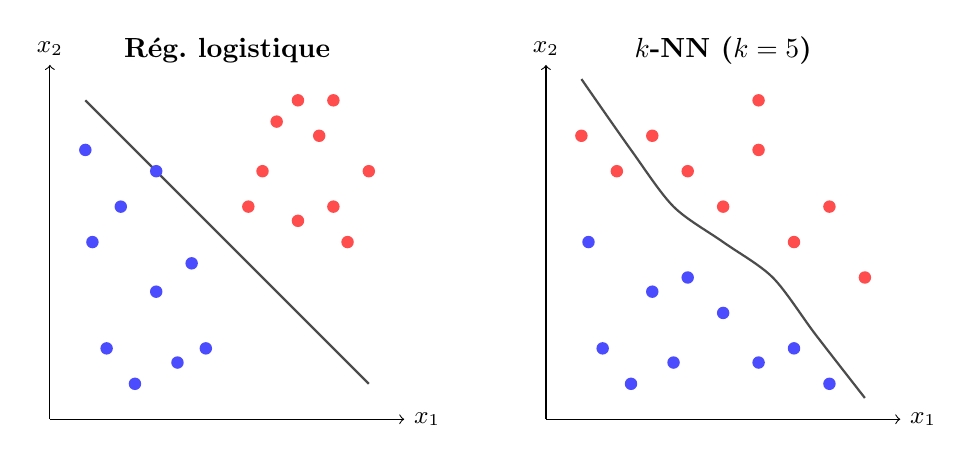
\begin{tikzpicture}[scale=0.9]
  % --- Regression logistique ---
  \begin{scope}[xshift=0cm]
    \node[font=\bfseries] at (2.5, 5.2) {R\'eg.\ logistique};
    \draw[->] (0,0) -- (5,0) node[right, font=\small]{$x_1$};
    \draw[->] (0,0) -- (0,5) node[above, font=\small]{$x_2$};
    % fronti\`ere lin\'eaire
    \draw[thick, black!70] (0.5,4.5) -- (4.5,0.5);
    % classe 0
    \foreach \x/\y in {0.8/1.0, 1.2/0.5, 1.5/1.8, 0.6/2.5, 1.8/0.8,
      2.0/2.2, 1.0/3.0, 1.5/3.5, 0.5/3.8, 2.2/1.0}{
      \fill[blue!70] (\x, \y) circle (2.5pt);
    }
    % classe 1
    \foreach \x/\y in {3.0/3.5, 3.5/2.8, 4.0/3.0, 3.8/4.0, 4.2/2.5,
      3.2/4.2, 4.0/4.5, 2.8/3.0, 3.5/4.5, 4.5/3.5}{
      \fill[red!70] (\x, \y) circle (2.5pt);
    }
  \end{scope}
  % --- k-NN ---
  \begin{scope}[xshift=7cm]
    \node[font=\bfseries] at (2.5, 5.2) {$k$-NN ($k=5$)};
    \draw[->] (0,0) -- (5,0) node[right, font=\small]{$x_1$};
    \draw[->] (0,0) -- (0,5) node[above, font=\small]{$x_2$};
    % fronti\`ere non-lin\'eaire
    \draw[thick, black!70, smooth] plot coordinates
      {(0.5,4.8) (1.2,3.8) (1.8,3.0) (2.5,2.5) (3.2,2.0) (3.8,1.2) (4.5,0.3)};
    % classe 0
    \foreach \x/\y in {0.8/1.0, 1.2/0.5, 1.5/1.8, 0.6/2.5, 1.8/0.8,
      2.5/1.5, 3.0/0.8, 3.5/1.0, 2.0/2.0, 4.0/0.5}{
      \fill[blue!70] (\x, \y) circle (2.5pt);
    }
    % classe 1
    \foreach \x/\y in {0.5/4.0, 1.0/3.5, 1.5/4.0, 2.0/3.5, 2.5/3.0,
      3.0/3.8, 3.5/2.5, 4.0/3.0, 4.5/2.0, 3.0/4.5}{
      \fill[red!70] (\x, \y) circle (2.5pt);
    }
  \end{scope}
\end{tikzpicture}
\caption{Fronti\`eres de d\'ecision : r\'egression logistique (lin\'eaire) vs.\ $k$-NN (non-lin\'eaire).}
\label{fig:decision-boundaries}
\end{figure}

% ============================================================
\section{\'Evaluation des classifieurs}
\label{sec:evaluation}

\subsection{Matrice de confusion}

\begin{definition}[Matrice de confusion -- cas binaire]
\[
  \begin{array}{c|cc}
    & \hat{y} = 1 & \hat{y} = 0 \\ \hline
    y = 1 & \text{VP} & \text{FN} \\
    y = 0 & \text{FP} & \text{VN}
  \end{array}
\]
o\`u VP = vrais positifs, FP = faux positifs, VN = vrais n\'egatifs, FN = faux n\'egatifs.
\end{definition}

\begin{formules}[title=\textbf{M\'etriques de classification}]
\begin{align*}
  \text{Pr\'ecision} &= \frac{\text{VP}}{\text{VP} + \text{FP}}, &
  \text{Rappel (Sensibilit\'e)} &= \frac{\text{VP}}{\text{VP} + \text{FN}} \\[4pt]
  \text{Sp\'ecificit\'e} &= \frac{\text{VN}}{\text{VN} + \text{FP}}, &
  F_1 &= \frac{2 \cdot \text{Pr\'ecision} \cdot \text{Rappel}}{\text{Pr\'ecision} + \text{Rappel}}
\end{align*}
\end{formules}

\subsection{Courbe ROC et AUC}

\begin{definition}[Courbe ROC]
La courbe ROC (\emph{Receiver Operating Characteristic}) trace le taux de vrais positifs
(rappel) en fonction du taux de faux positifs ($1 - \text{sp\'ecificit\'e}$) pour
diff\'erents seuils de d\'ecision $\tau \in [0, 1]$.

L'\textbf{AUC} (\emph{Area Under the Curve}) mesure la qualit\'e globale du classifieur :
\[
  \text{AUC} = P(\hat{p}_{Y=1} > \hat{p}_{Y=0}) = \int_0^1 \text{TPR}(\tau)\, d\text{FPR}(\tau)
\]
Un classifieur al\'eatoire a $\text{AUC} = 0.5$, un classifieur parfait a $\text{AUC} = 1$.
\end{definition}

% ============================================================
\section{Impl\'ementation Python}
\label{sec:classif-python}

\subsection{R\'egression logistique}

\begin{codeblock}[title=\textbf{R\'egression logistique depuis z\'ero}]
\begin{minted}{python}
import numpy as np

class LogisticRegressionScratch:
    def __init__(self, lr=0.1, n_iter=1000):
        self.lr = lr
        self.n_iter = n_iter

    def _sigmoid(self, z):
        return 1 / (1 + np.exp(-np.clip(z, -500, 500)))

    def fit(self, X, y):
        n, p = X.shape
        self.w_ = np.zeros(p)
        self.b_ = 0.0
        self.losses_ = []

        for _ in range(self.n_iter):
            z = X @ self.w_ + self.b_
            p_hat = self._sigmoid(z)
            # Gradient
            dw = -(1/n) * X.T @ (y - p_hat)
            db = -(1/n) * np.sum(y - p_hat)
            self.w_ -= self.lr * dw
            self.b_ -= self.lr * db
            # Log-loss
            loss = -np.mean(
                y * np.log(p_hat + 1e-15)
                + (1 - y) * np.log(1 - p_hat + 1e-15)
            )
            self.losses_.append(loss)
        return self

    def predict_proba(self, X):
        return self._sigmoid(X @ self.w_ + self.b_)

    def predict(self, X, threshold=0.5):
        return (self.predict_proba(X) >= threshold).astype(int)
\end{minted}
\end{codeblock}

\subsection{Les trois classifieurs avec scikit-learn}

\begin{codeblock}[title=\textbf{Logistique, $k$-NN et Na\"ive Bayes -- scikit-learn}]
\begin{minted}{python}
from sklearn.linear_model import LogisticRegression
from sklearn.neighbors import KNeighborsClassifier
from sklearn.naive_bayes import GaussianNB
from sklearn.model_selection import (
    train_test_split, cross_val_score
)
from sklearn.metrics import (
    classification_report, confusion_matrix,
    roc_curve, roc_auc_score
)
from sklearn.datasets import make_classification
from sklearn.preprocessing import StandardScaler
import numpy as np
import matplotlib.pyplot as plt

# --- Donnees synthetiques ---
X, y = make_classification(
    n_samples=500, n_features=2,
    n_informative=2, n_redundant=0,
    random_state=42
)
X_train, X_test, y_train, y_test = train_test_split(
    X, y, test_size=0.3, random_state=42
)
scaler = StandardScaler()
X_train_s = scaler.fit_transform(X_train)
X_test_s = scaler.transform(X_test)

# --- Modeles ---
models = {
    "Logistique": LogisticRegression(),
    "k-NN (k=5)": KNeighborsClassifier(n_neighbors=5),
    "Naive Bayes": GaussianNB()
}

for name, model in models.items():
    model.fit(X_train_s, y_train)
    y_pred = model.predict(X_test_s)
    acc = np.mean(y_pred == y_test)
    cv_scores = cross_val_score(
        model, X_train_s, y_train, cv=5
    )
    print(f"--- {name} ---")
    print(f"Accuracy test : {acc:.3f}")
    print(f"CV accuracy   : {cv_scores.mean():.3f} "
          f"(+/- {cv_scores.std():.3f})")
    print(confusion_matrix(y_test, y_pred))
    print()
\end{minted}
\end{codeblock}

\begin{codeoutput}
\begin{minted}{text}
--- Logistique ---
Accuracy test : 0.893
CV accuracy   : 0.886 (+/- 0.025)
[[68  7]
 [ 9 66]]

--- k-NN (k=5) ---
Accuracy test : 0.880
CV accuracy   : 0.871 (+/- 0.031)
[[65 10]
 [ 8 67]]

--- Naive Bayes ---
Accuracy test : 0.887
CV accuracy   : 0.877 (+/- 0.028)
[[67  8]
 [ 9 66]]
\end{minted}
\end{codeoutput}

\begin{codeblock}[title=\textbf{Courbe ROC comparative}]
\begin{minted}{python}
plt.figure(figsize=(7, 5))
for name, model in models.items():
    if hasattr(model, "predict_proba"):
        y_score = model.predict_proba(X_test_s)[:, 1]
    else:
        y_score = model.decision_function(X_test_s)
    fpr, tpr, _ = roc_curve(y_test, y_score)
    auc = roc_auc_score(y_test, y_score)
    plt.plot(fpr, tpr, label=f"{name} (AUC={auc:.3f})")

plt.plot([0, 1], [0, 1], 'k--', label="Aleatoire")
plt.xlabel("Taux de faux positifs")
plt.ylabel("Taux de vrais positifs")
plt.title("Courbes ROC")
plt.legend()
plt.tight_layout()
plt.savefig("roc_comparison.pdf")
plt.show()
\end{minted}
\end{codeblock}

% ============================================================
\section{Exercices}
\label{sec:classif-exercices}

\begin{exercice}[Niveau 1 -- R\'egression logistique \`a la main]
On consid\`ere un probl\`eme binaire avec une seule variable $x$ et les param\`etres
$w = 2$, $b = -3$.
\begin{enumerate}
  \item Calculer $P(Y = 1 \mid x)$ pour $x \in \{0, 1, 1.5, 2, 3\}$.
  \item D\'eterminer la fronti\`ere de d\'ecision (pour $\tau = 0.5$).
  \item On observe $(x_1, y_1) = (1, 0)$ et $(x_2, y_2) = (2, 1)$. Calculer
        la log-vraisemblance $\ell(w, b)$.
  \item Calculer le gradient $\nabla_{(w,b)} \mathcal{L}$ pour ces deux observations.
\end{enumerate}
\end{exercice}

\begin{exercice}[Niveau 2 -- Comparaison exp\'erimentale]
Charger le jeu de donn\'ees \texttt{Iris} (3 classes, 4 variables).
\begin{enumerate}
  \item S\'eparer en 70\% entra\^inement / 30\% test.
  \item Entra\^iner les trois classifieurs (r\'egression logistique multiclasse,
        $k$-NN avec $k \in \{1, 3, 5, 7, 11\}$, Na\"ive Bayes gaussien).
  \item Afficher les matrices de confusion et les rapports de classification.
  \item Pour $k$-NN, tracer l'accuracy de validation crois\'ee en fonction de $k$.
        Quel $k$ est optimal ?
  \item Visualiser les fronti\`eres de d\'ecision en 2D (sur les deux premi\`eres
        composantes principales).
\end{enumerate}
\end{exercice}

\begin{exercice}[Niveau 3 -- Analyse th\'eorique]
\begin{enumerate}
  \item Montrer que la fonction de co\^ut de la r\'egression logistique est convexe.
        \emph{Indication :} calculer la hessienne $\bm{H} = \bm{X}^\top \bm{S} \bm{X}$
        o\`u $\bm{S} = \text{diag}(\hat{p}_i(1-\hat{p}_i))$ et montrer qu'elle est
        semi-d\'efinie positive.
  \item D\'emontrer que le classifieur bay\'esien optimal $h^*(\bm{x}) = \argmax_k P(Y=k \mid \bm{x})$
        minimise le risque $R(h) = P(h(\bm{X}) \neq Y)$.
  \item Pour le Na\"ive Bayes gaussien avec deux classes \'equiprobables et $\sigma_{j0} = \sigma_{j1} = \sigma_j$,
        montrer que la fronti\`ere de d\'ecision est un \textbf{hyperplan} (fronti\`ere lin\'eaire).
        En d\'eduire le lien avec la r\'egression logistique.
  \item Montrer que le taux de convergence du $k$-NN est
        $\E[R(\hat{h}_k)] - R(h^*) = O(n^{-2/(2+p)})$ et commenter le fl\'eau
        de la dimension.
\end{enumerate}
\end{exercice}
